\documentclass[../Dissertation.tex]{subfiles}

\begin{document}

\subsection{Overview}
\emph{
\begin{itemize}
	\item Questions to be addressed
	\item Metrics to be measured - why
\end{itemize}
}
\subsection{Conceptual Process}
\emph{
\begin{itemize}
	\item Sensitivity analysis - filter/channel selection and layer interdependencies
	\item Filter pruning implementation - Theory
	\item Channel pruning implementation - Theory
	\item Retraining pruned model
\end{itemize}
}

\subsection{Filter and channel selection}
\emph{
Link back to selected model - concrete examples of process described in previous section
\begin{itemize}
	\item Filter selection (visual representation of filters)
	\item Channel selection (visual representation of channels)
	\item Discussion of pruning consequences (and recovery) -> top1/top5 before retraining and after
\end{itemize}
}

\subsection{Engineering/implementation details}
\emph{
\begin{itemize}
	\item High level overview of physical system - justify need for multiple training agents
    \item Pruning \& retraining setup - Distiller (Pruning \& training)
	\item Benchmarking setup - openvino + benchmark (getting latency/throughput)
	\item Data processing - wandb + data visualisation steps
\end{itemize}
}

\subsubsection{High level overview of system}

\begin{figure}[H]
    \centering
    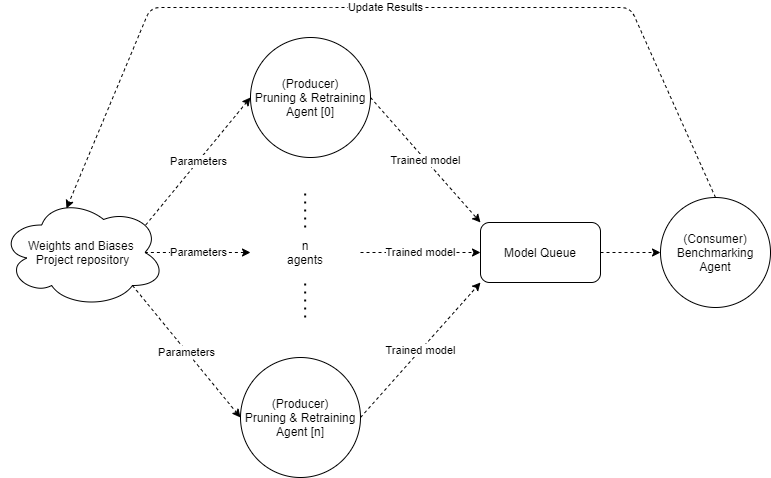
\includegraphics[width=\textwidth]{./ProducerConsumer}
    \caption{Diagram showing agent communication}
    \label{fig:agentCommunication}
\end{figure}

While the process of pruning is relatively fast, retraining the network to regain lost accuracy can very demanding. To handle this problem we separated the benchmarking system (consumer) from the pruning and retraining systems (producer), this made it easy to add new pruning and benchmarking agents to a single experiment or run multiple experiments in parallel.

When pruning begins, the producer agent requests the (initially random) pruning parameters from the Weights and Biases Project server, the producer then applies the pruning algorithm and begins retraining the model. Upon completion of retraining the model is exported into ONNX format and added to a queue for the consumer (the benchmarking agent) to benchmark and record the results, these results are then logged to weights and biases.

\subsubsection{defining parameters to prune}

Distiller uses a compression schedule yaml document to define the filters and channels to prune.

The pruning schedule is composed of lists of sections that define Pruners, LR-schedulers, and policies. A Pruner defines a pruning algorithm and the layers on which that pruning algorithm will be applied, LR-schedulers define the \textbf{learning-rate decay(Definition required)} algorithm. 
Finally each policy defines the instance of the pruner or LR-scheduler it is managing, define when the respective algorithm will be applied, such as the start and end epoch, and the frequency of application.

Each layer in the network is labelled internally by Pytorch, distiller uses these labels to identify the layers being referenced by the compression schedule, 

\subsubsection{Benchmarking}

\begin{figure}[H]
	\centering
	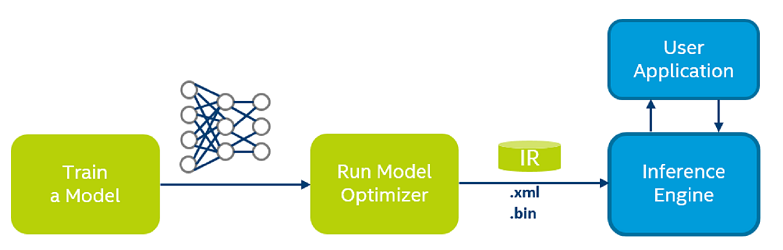
\includegraphics{./OpenVinoModelOptimizer}
	\caption{Workflow for deploying trained model onto NCS \autocite{ModelOptimizerDeveloper}}
	\label{fig:OpenVinoWorkflow}
\end{figure}


To pass the pruned and trained model to the Neural Compute stick we used OpenVino; a toolkit providing a high level \textbf{inference engine(Ensure this is defined)} API, this facilitates the process of optimizing the model for specialised hardware (in this case the NCS). 
OpenVino itself has a Benchmarking tool that we leverage to access to detailed latency and throughput metrics. A predefined set of images are selected and loaded into the NCS, the benchmarking application then runs 100 iterations by passing the same 4 images through the network and returns the mean end-to-end latency (including loading images into the NCS memory), VPU processing latency (Inference latency), and throughput in FPS.


\end{document}